\hspace{0.5cm} Oil spill detection can be done with several methods. In the field of optical imaging alone, there are plenty of options. Aircrafts can create images across various spectra of light with different cameras. Laser fluorsensors measure the emission fluorescent light when oil hit by ultraviolet light \cite{fingas2014review}. Synthetic Aperture Radar(SAR) image has a high resolution, wide area coverage and moreover images can be taken day and night under any weather condition. This enables oil spill investigators to monitor oceans 24 hours a day\cite{Chang20081915}. The advantage of this is that large areas can be checked for spills, which is often required when checking oceans. The main alternative within radar imaging is Side-Looking Airborne Radar, which is an older but significantly cheaper method \cite{fingas2014review}. 

SAR images are created through radio waves. Radio waves are sent from the SAR device to an area. That area reflects radio waves in a certain way, which is measured through the time the waves take to travel back. \cite{Doerry:04} When an ocean is hit by radio waves, those waves are reflected in a certain way. Oil reflects radio waves in a different way. This difference is the key to identifying oil spills.

An overview for the oil spill detection approach is shown in Fig. 1, these are the basic steps independent of the chosen classifier.

\begin{figure}[H]
    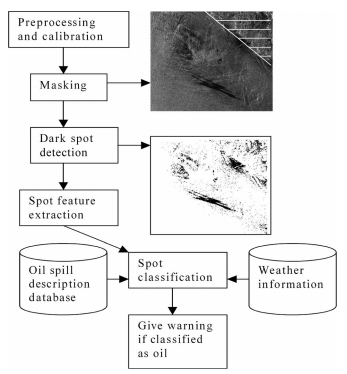
\includegraphics[width=80mm]{./img/detection_diagram.png}
    \caption{Overview for the oil spill detection approach \cite{Solberg200745}}
    \label{fig:overview}
\end{figure}






